\documentclass[paper=a4,fontsize=12pt,ngerman]{scrartcl}

\usepackage[utf8]{inputenc}				
\usepackage[T1]{fontenc}
\usepackage{graphicx}
\usepackage[ngerman]{babel}
\usepackage{amsmath}
\usepackage{url}
\usepackage{hyperref}
\usepackage[a4paper,left=25mm,right=35mm,top=25mm,bottom=30mm]{geometry}
\usepackage{parskip}
\usepackage{listings}
\usepackage{color}

\lstset{
    basicstyle=\ttfamily\small,
    frame=single,
    breaklines=true,
    language=,
    captionpos=b
}

\begin{document}

\pagenumbering{roman}
\pagestyle{plain}

% Einbinden der Titelseite
\begin{titlepage}

\linespread{1.5}


\includegraphics[width=\linewidth]{graphics/htw_logo}

\begin{center}
    \large  
    \hfill
    \vfill
    \Large{\bfseries{Handflächenzahlung in China: Technik und Sicherheit}}
    
    von \\
    Xudong Zhang \\
    Matrikelnummer: 5014211\\

    \vfill
		
    Ein wissenschaftlicher Bericht im Rahmen der Vorlesung\\
    \glqq Wissenschaftliches Arbeiten\grqq\\
    an der htw saar im Studiengang Informatik\\
	
    \vfill	
    \vfill
	
    Saarbrücken, den 06.08.2025
\end{center}
    
\end{titlepage}


% Hier ist der Abstract
\section*{Abstract}
In dieser Arbeit wird die neue Handflächenerkennung von WeChat vorgestellt und bewertet. Die Technologie nutzt die Linien und Venen der Hand, um Zahlungen sicher und ohne Berührung durchzuführen. Die Handflächenerkennung ist sicherer, schneller und hygienischer als andere Methoden wie QR-Code, Fingerabdruck oder Gesichtserkennung.


\newpage
\section*{Selbstständigkeitserklärung}
Ich versichere, dass ich die vorliegende Arbeit selbstständig verfasst und 
keine anderen als die angegebenen Quellen und Hilfsmittel benutzt habe.
Insbesondere habe ich alle KI-basierten Werkzeuge angegeben, die ich bei
der Erstellung, Übersetzung oder Überarbeitung des Textes verwendet habe.

Ich erkläre hiermit weiterhin, dass die vorgelegte Arbeit zuvor weder von mir 
noch von einer anderen Person an dieser oder einer anderen Hochschule 
eingereicht wurde.

Darüber hinaus ist mir bekannt, dass die Unrichtigkeit dieser Erklärung eine 
Benotung der Arbeit mit der Note \glqq nicht ausreichend\grqq \ zur Folge hat 
und einen Ausschluss von der Erbringung weiterer Prüfungsleistungen zur Folge 
haben kann.
\bigskip
 
Saarbrücken, den 06.08.2025

\smallskip
Xudong Zhang




% Das Inhaltsverzeichnis
\clearpage
\tableofcontents 

\clearpage
\pagenumbering{arabic}


\section{Einleitung}
Physische Karten können leicht verloren gehen. Beim mobilen Bezahlen kommt es vor, dass der Akku des Smartphones leer ist. In Zeiten von Grippewellen kann die Nutzung von Fingerabdruckscannern zudem hygienische Risiken mit sich bringen.\cite{tencent2024article}

Heute gibt es jedoch eine neue Entwicklung im Bereich des Bezahlens: Eine einfache Handbewegung genügt, um eine Zahlung oder Identitätsprüfung durchzuführen und einen Dienst zu nutzen.

Die Handflächenerkennung, die von \textbf{WeChat} eingeführt wurde, verbessert den Alltag deutlich. Sie erhöht sowohl den Komfort als auch die Sicherheit.


\subsection{Grundlagen und Begriffe}

Vor der Einführung der \textbf{Handflächenerkennung} durch WeChat gab es bereits 
verschiedene biometrische und technologische Zahlungsmethoden, wie z. B. QR-Codes, 
Fingerabdruck- und Gesichtserkennung. Jede dieser Methoden hatte jedoch ihre eigenen 
Einschränkungen.

\begin{table}[h]
\centering
\begin{tabular}{|l|p{5cm}|p{5cm}|}
\hline
\textbf{Methode} & \textbf{Vorteile} & \textbf{Nachteile} \\ 
\hline
QR-Code & Weit verbreitet, einfach & Gerät nötig, zeitaufwändig \\
\hline
Fingerabdruck & Schnell, sicher & Hygienisch problematisch \\
\hline
Gesichtserkennung & Kontaktlos, bequem & Lichtabhängig, Datenschutz \\
\hline
\end{tabular}
\caption{Vergleich mobiler Zahlungsmethoden}
\label{tab:zahlungsmethoden}
\end{table}

Die \textbf{Handflächenerkennung} bietet eine Lösung für diese Herausforderungen.
Eine vielversprechende Alternative, die genauer und stabiler ist.\cite{tang2022wechat}. 

\vspace*{1.5cm}

\subsection{Definitionen}
\textbf{Biometrische Authentifizierung} heißt, dass die Identität anhand von körperlichen Merkmalen wie Fingerabdruck, Gesicht, Stimme oder Iris überprüft wird. Weil diese Merkmale bei jedem Menschen anders sind, können sie benutzt werden, um die Identität einer Person zu überprüfen. \cite{geeksforgeeks2025palm}

\textbf{Handflächenerkennung} ist ein Verfahren, das die Hand scannt, um ein eindeutiges Muster zu finden. Es soll eine Identifikation ermöglicht werden. \cite{innovatrics2025palm}

\textbf{WeChat Handflächen-Zahlung}  ist ein System von Tencent. Es erkennt die Handflächen der Nutzer und ermöglicht so sichere und kontaktlose Zahlungen. \cite{tencent2024palm}

\vspace{2cm}

\section{Analyse und Bewertung}

\subsection{Technische Funktionsweise}
Die \textbf{WeChat-Handflächenerkennung} basiert auf einer innovativen doppelten 
biometrischen Technologie, die zwei verschiedene Erkennungsverfahren kombiniert:

\textbf{Duale Bilderfassung}: Das System nutzt sowohl Farbbilder als auch 
Infrarotaufnahmen, um ein umfassendes biometrisches Profil zu erstellen. Diese 
Kombination ermöglicht eine gleichzeitige Analyse verschiedener Handmerkmale:

\begin{figure}[h]
\begin{center}
  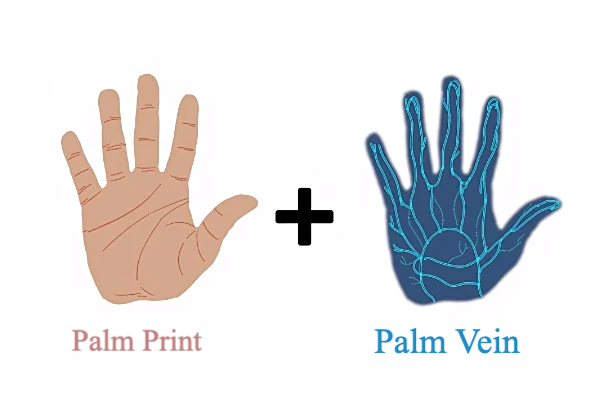
\includegraphics[scale=0.35]{graphics/palm.png}
  \caption{Handflächenerkennung}
  \label{handfläche}
\end{center}
\end{figure}

\begin{itemize}
\item \textbf{Handlinien-Analyse (Palm Print)}: Digitale Erfassung der natürlichen 
Linienführung und Oberflächenstruktur der Handfläche mittels hochauflösender 
Farbkameras
\item \textbf{Handvenenstruktur (Palm Vein)}: Infrarotscanner erfassen das 
einzigartige Muster der Blutgefäße unter der Hautoberfläche
\end{itemize}

\textbf{Erweiterte Sicherheitsmerkmale}: WeChat verwendet zusätzliche 
Verifikationsebenen zur Betrugsverhinderung:
\begin{itemize}
\item Erkennung künstlicher Hände oder Handabdrücke
\item Verhinderung der Nutzung fremder Hände
\item Unterscheidung selbst bei eineiigen Zwillingen möglich
\item Bestätigung der physischen Anwesenheit und freiwilligen Durchführung
\end{itemize}

Die Kombination dieser Merkmale ermöglicht laut WeChat Pay eine 
Erkennungsgenauigkeit von über 99,9\% und macht Fälschungen nahezu 
unmöglich \cite{pan2024palm}. Der dreifache Sicherheitsansatz aus Handlinien, 
Venenstruktur und Lebenderkennung stellt sicher, dass nur die berechtigte 
Person selbst eine Transaktion durchführen kann.\cite{haoMiao2025wechat}

\textbf{Fusion von Handlinien- und Handvenenmerkmalen}: Nachdem die Informationsgewichte $W_1$ und $W_2$ für die beiden Modalitäten Handlinien und Handvenen bestimmt wurden, wird $W_1$ als Gewicht mit der konvolutionellen Merkmalskarte $P_2$ der Handlinienbilder multipliziert, um $P_3$ zu erhalten. Ebenso wird $W_2$ mit der konvolutionellen Merkmalskarte $V_2$ der Handvenenbilder multipliziert, um $V_3$ zu erhalten. Dieser Vorgang wird durch die folgenden Gleichungen beschrieben:


\begin{equation}
P_3 = W_1 \cdot P_2,\quad V_3 = W_2 \cdot V_2
\end{equation}

Mit dieser flexiblen Fusionsmethode kann das Modell besser auf Unterschiede zwischen den einzelnen Erkennungsmerkmalen und auf unterschiedliche Bildqualitäten reagieren. Dadurch entsteht eine stabilere und zuverlässigere gemeinsame Merkmalsdarstellung. Im nächsten Schritt werden die Merkmalskarten $P_3$ (Handlinien) und $V_3$ (Handvenen) einfach zusammengefügt, sodass die endgültige Merkmalskarte $Z$ entsteht. Die entsprechende Formel lautet:

\begin{equation}
Z = \text{Concate}[P_3, V_3]
\end{equation}
Das Wort $Concate$ steht hier für das Verketten der beiden Merkmalskarten. Die so entstandene konvolutionelle Merkmalskarte $Z$ wird anschließend in eine vollständig verbundene Schicht weitergeleitet, um die Identität zu bestimmen. Für die Bewertung des Netzwerks wird die sogenannte Kreuzentropie-Verlustfunktion verwendet, die wie folgt berechnet wird:

\begin{equation}
L_{\text{CLS}} = -\sum_{i=1}^{k} y_i \cdot \log(q_i')
\end{equation}

Hierbei bezeichnet $q$ das Klassifikationsergebnis, das nach der Einspeisung der konvolutionellen Merkmalskarte $Z$ in die vollständig verbundene Schicht erhalten wird. Das Label $y$ gibt die tatsächliche Klasse der multimodalen konvolutionellen Merkmalskarte $Z$ an.

Die Gesamtverlustfunktion des Netzwerkrahmens wird wie folgt berechnet:

\begin{equation}
L = \lambda_1 \cdot L_1 + \lambda_2 \cdot L_{m}^{ZF} + \lambda_3 \cdot L_{\text{CLS}}
\end{equation}

Hier sind $\lambda_1$, $\lambda_2$, $\lambda_3$ Hyperparameter, die die einzelnen Verlustfunktionen gewichten.

Durch diese mathematische Struktur kann das System Personen sehr zuverlässig und sicher erkennen, sodass Fälschungen praktisch ausgeschlossen sind.\cite{pan2024palm}

\vspace{1.5cm}

\subsection{Herausforderungen und Limitationen}
Trotz der modernen Technik hat die WeChat-Handflächenerkennung einige Herausforderungen:

\textbf{Teure Hardware}: Das System braucht spezielle Geräte mit besonderen 
Kameras. Normale Handys können nicht benutzt werden. Die Technik ist teuer.

\textbf{Schwierige Anmeldung}: Neue Nutzer müssen ihre Hand registrieren. 
Das dauert länger als bei QR-Codes.

\textbf{Datenschutz-Probleme}: Das System speichert Körperdaten, die sehr sensible sind. 
Viele Menschen haben Angst vor Missbrauch.

\vspace{1.5cm}



\vspace{2cm}

\section{Ergebnisse und Diskussion}

\subsection{Experimentelle Validierung der Fusionsmethoden}
Um die vorgestellten Methoden zu überprüfen, wurden verschiedene multimodale Fusionsalgorithmen in praktischen Tests miteinander verglichen. Die Ergebnisse zeigen, dass moderne Fusionsverfahren besonders zuverlässig und leistungsfähig sind.

\begin{figure}[h!]
\begin{center}
  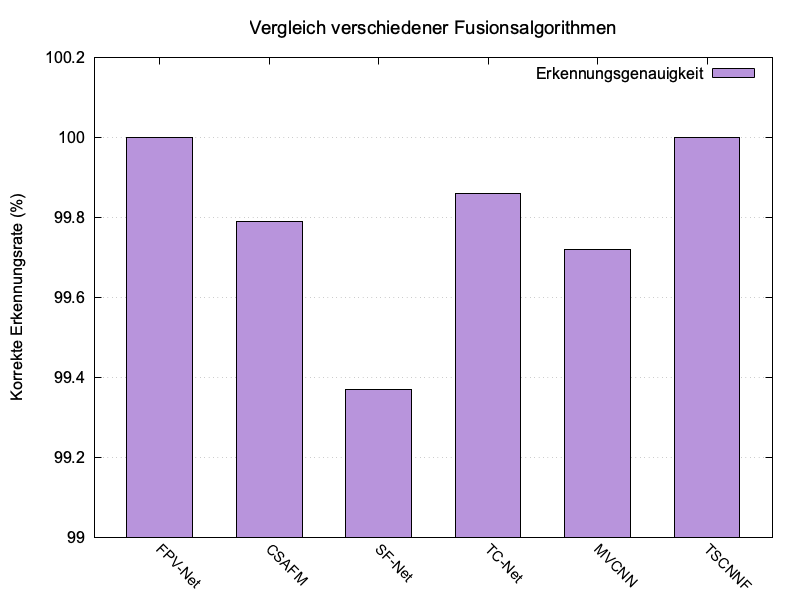
\includegraphics[width=0.7\textwidth]{graphics/fusion_algorithms_comparison.png}
  \caption{Vergleich verschiedener Fusionsalgorithmen}
  \label{fig:fusion-comparison}
\end{center}
\end{figure}

Abbildung \ref{fig:fusion-comparison} zeigt die Ergebnisse verschiedener Fusionsmethoden. Besonders die FPV-Net und TSCNNF erreichen eine sehr hohe Erkennungsrate von 100\%. Dadurch wird bestätigt, dass der kombinierte Ansatz besser funktioniert als einzelne Verfahren.\cite{pan2024palm}

\vspace{1.5cm}

\subsection{Leistungsvergleich mit bestehenden Systemen}
Im Vergleich zu traditionellen Zahlungsmethoden hat die Handflächenerkennung mehrere klare Vorteile. Sie ist besonders sicher, da sie nur schwer zu fälschen ist. Außerdem funktioniert sie kontaktlos, was hygienischer ist und schneller geht. Die folgende Tabelle zeigt die wichtigsten Unterschiede zu anderen biometrischen Verfahren:

\begin{table}[!htb]
\centering
\begin{tabular}{|l|c|c|c|}
\hline
\textbf{Kriterium} & \textbf{Handflächen} & \textbf{Fingerabdruck} & \textbf{Gesicht} \\
\hline
Genauigkeit & 99,9\% & 95-98\% & 92-96\% \\
\hline
Kontaktlos & Ja & Nein & Ja \\
\hline
Hygienisch & Sehr gut & Problematisch & Gut \\
\hline
Fälschungsresistenz & Sehr hoch & Mittel & Niedrig-Mittel \\
\hline
Lichtabhängigkeit & Gering & Keine & Hoch \\
\hline
Geschwindigkeit & 0,3-0,5s & 0,5-1s & 1-2s \\
\hline
Hardware-Kosten & Hoch & Niedrig & Mittel \\
\hline
Datenschutz & Mittel & Gut & Problematisch \\
\hline
\end{tabular}
\caption{Leistungsvergleich biometrischer Erkennungsverfahren}
\label{tab:biometric-comparison}
\end{table}

In der Tabelle \ref{tab:biometric-comparison} sieht man, dass die \textbf{Handflächenerkennung} bei fast allen Kriterien besser ist als andere biometrische Verfahren. Besonders wichtig sind die sehr hohe Erkennungsgenauigkeit (99,9\%) und die kontaktlose Nutzung, die für mehr Sicherheit und Hygiene sorgen.


\vspace{2cm}

\section{Fazit und Schlussfolgerungen}
Die Handflächenerkennung von WeChat stellt einen bedeutenden Fortschritt in der biometrischen Zahlungstechnologie dar. Die duale Erfassung von Handlinien und Handvenen erreicht eine Erkennungsgenauigkeit von 99,9\% und übertrifft damit etablierte Methoden deutlich.

Die wichtigsten Erkenntnisse dieser Arbeit:

\textbf{Technische Überlegenheit}: Die multimodale Fusionstechnik kombiniert erfolgreich verschiedene biometrische Merkmale und erreicht höchste Sicherheitsstandards.

\textbf{Praktische Vorteile}: Kontaktlose Bedienung, schnelle Transaktionszeiten (0,3-0,5s) und hohe Hygienestandards machen das System besonders attraktiv.

\textbf{Herausforderungen}: Hohe Hardwarekosten und Datenschutzbedenken stellen noch immer Hindernisse für eine breite Einführung dar.

Die Handflächenerkennung hat großes Potenzial. Und zwar für die Zukunft des digitalen Bezahlens. Insbesondere in öffentlichen Bereichen mit hohem Durchsatz.

\vspace{1.5cm}

\subsection{Offene Fragen}
\begin{itemize}
  \item Wie kann die Technologie kostengünstiger und für mobile Geräte verfügbar gemacht werden?
  \item Welche rechtlichen Standards sind für biometrische Zahlungssysteme erforderlich?
  \item Wie entwickelt sich die gesellschaftliche Akzeptanz dieser Technologie?
  \item Welche Langzeiteffekte haben Hautveränderungen auf die Erkennungsqualität?
\end{itemize}

\vspace{1.5cm}

\subsection{Diskussion}
Die Innovation von WeChat zeigt, wie zukünftige Zahlungssysteme aussehen könnten. Damit sich diese Technik wirklich durchsetzt, müssen nicht nur die technischen Vorteile überzeugen, sondern auch die gesellschaftlichen und wirtschaftlichen Aspekte.

Künftige Forschung sollte darauf abzielen, die Kosten zu senken. Außerdem sollte sie den Datenschutz weiter verbessern. So wird diese moderne Technologie für möglichst viele Menschen nutzbar.

% Hier beginnt das Literaturverzeichnis
\clearpage
\renewcommand\refname{Literaturverzeichnis}
\bibliographystyle{alpha}
\bibliography{literatur}
\addcontentsline{toc}{section}{Literaturverzeichnis}


\clearpage
\appendix
\part*{Anhang}
\addcontentsline{toc}{section}{Anhang}

\section{GNUplot-code}
\begin{lstlisting}[caption={Gnuplot-Skript für Fusionsalgorithmen}]
#!/usr/bin/gnuplot

# Set terminal and output
set terminal pngcairo enhanced font "Arial,12" size 800,600
set output "graphics/fusion_algorithms_comparison.png"

# Set title and labels
set title "Vergleich verschiedener Fusionsalgorithmen" font "Arial,14"
set ylabel "Korrekte Erkennungsrate (%)" font "Arial,12"
set xlabel "" font "Arial,12"

# Set y-axis range to focus on the differences
set yrange [99:100.2]

# Set grid
set grid y

# Set bar chart style
set style fill solid 0.7 border -1
set boxwidth 0.6

# Set x-axis labels
set xtics rotate by -45 font "Arial,11"

# Set colors for different performance levels
set style data histograms
set style histogram cluster gap 1

# Define color palette: purple for 100%, blue for high performance, teal for good, orange for lower
plot 'fusion_data.dat' using 2:xtic(1) with boxes \
     lc rgb "#9966CC" title "Erkennungsgenauigkeit"
\end{lstlisting}


\section{Website Ressourcen}

\begin{itemize}
  \item \url{https://www.gnuplot.info/} - Offizielle GNUplot-Website
  \item \url{http://www.gnuplotting.org/} - GNUplot Tutorials und Beispiele
  \item \url{https://www.overleaf.com/} - Online LaTeX Editor
  \item \url{https://www.deepl.com/} - Deepl Übersetzungsdienst
\end{itemize}

\end{document}
